\documentclass[10pt]{article}
\usepackage{graphicx}
\usepackage{extsizes}
\usepackage{multicol}
\usepackage{multirow}
\title{July2023 CSE300 Week10 Online Evaluation}
\author{Md. Emamul Haque Pranta}
\date{February 6, 2024}

\begin{document}

\maketitle
\tableofcontents
\pagebreak
\section{RISC Architecture}
\begin{figure}[h]
    \centering
    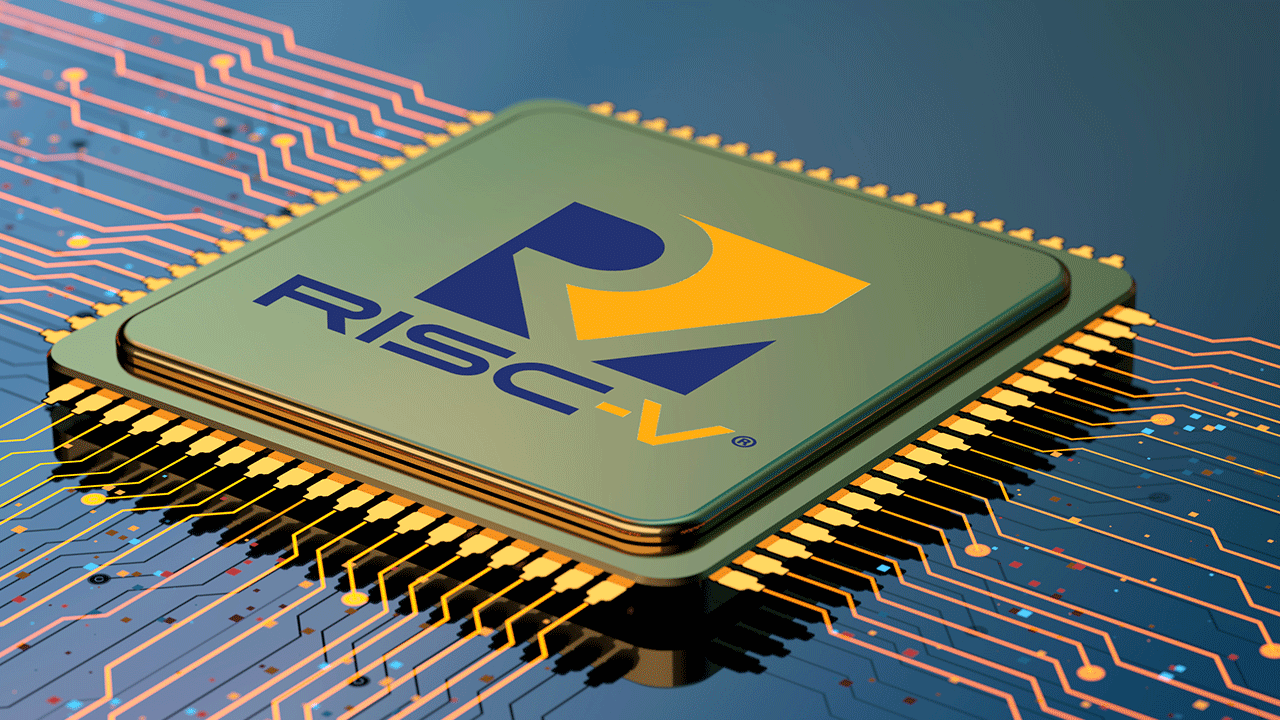
\includegraphics[scale=0.2]{Image/risc.png}
    \caption{RISC Architecture}
    \label{fig:enter-label}
\end{figure}
\section{Tables is \LaTeX}
\begin{table}[h]
    \centering
    \begin{tabular}{|c|c|c|c|}
    \hline
        \multirow{10}{*}{numeric literals}&\multirow{5}{*}{integers}&in decimal&8743\\
        \cline{3-4}
        &&\multirow{2}{*}{in octal}&0o7464\\
        \cline{4-4}
        &&&00103\\
        \cline{3-4}
        &&\multirow{2}{*}{in hexadecimal}&0x5A0FF\\
        \cline{4-4}
        &&&0xE0F2\\
        \cline{2-4}
        &\multirow{5}{*}{fractionals}&\multirow{5}{*}{in decimal}&140.58\\
        \cline{4-4}
        &&&8.04e7\\
        \cline{4-4}
        &&&0.347E+12\\
        \cline{4-4}
        &&&5.47E-12\\
        \cline{4-4}
        &&&47e22\\
        \hline
    \end{tabular}
    \caption{A table in \LaTeX}
    \label{tab:my_label}
\end{table}
Table \ref{tab:my_label} shows a table that contains cells spanning multiple columns and multiple rows.\cite{spec}
\pagebreak
\section{Writing Equations in Latex}
\begin{equation}
    L_{split}=\frac{1}{2}\left[\frac{G_L^2}{H_L+\lambda}+\frac{G_R^2}{H_R+\lambda}-\frac{(G_L+G_R)}{H_L+H_R+\lambda}\right]-\gamma
\end{equation}
Equation 1 has displayed above.\cite{spec2}
\section*{Untitled Section}
You need to display this section in your output PDF file. This section contains information
that may help you prepare the bibliography section. By the way, this section will not
show up in the table of contents.
    \begin{enumerate}
    \item Citation about the Greedy Forest Article

    \begin{itemize}
        \item \textbf{Authors: }T. Zhang, R. Johnson
        \item \textbf{Title: }Learning nonlinear functions using regularized greedy forest
        \item \textbf{Year: }2014
        \item \textbf{Journal: }IEEE Transactions on Pattern Analysis and Machine Intelligence
    \end{itemize}
    \item Citation about the Random Forest Article
    \begin{itemize}
        \item \textbf{Authors: }L. Breiman
        \item \textbf{Title: }Random Forests
        \item \textbf{Journal: }Machine Learning
        \item \textbf{Year: }2001
    \end{itemize}

    \end{enumerate}
    \bibliographystyle{acm}
    \bibliography{2005102}

\end{document}
